\begin{figure}[H]\centering
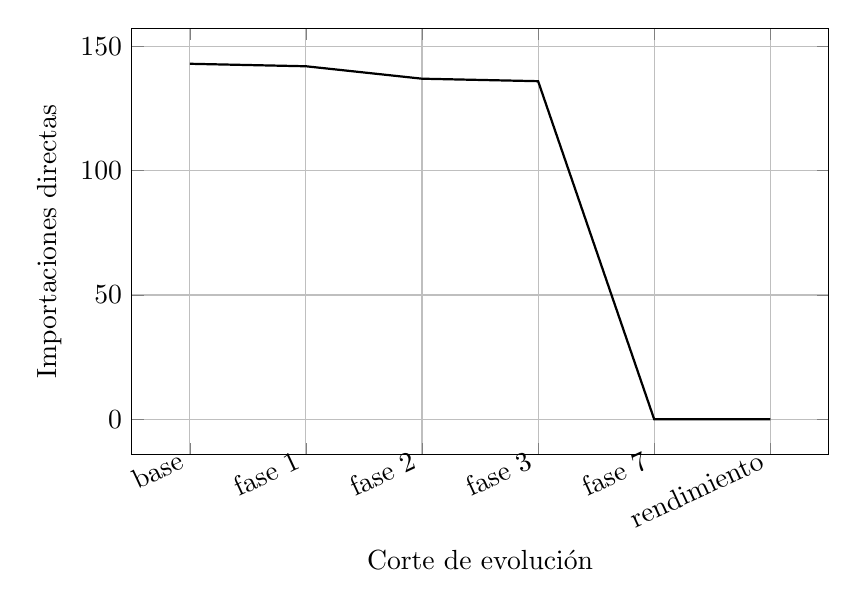
\begin{tikzpicture}\begin{axis}[width=.86\textwidth,height=7cm,xlabel={Corte de evolución},ylabel={Importaciones directas},xtick={0,1,2,3,4,5},xticklabels={base,fase 1,fase 2,fase 3,fase 7,rendimiento},x tick label style={rotate=25,anchor=east},grid=major,mark=*]
\addplot[black,thick] coordinates {(0,143) (1,142) (2,137) (3,136) (4,0) (5,0)};\end{axis}\end{tikzpicture}
\caption{Evolución longitudinal de accesos directos desde presentación. La figura se genera desde el historial analizado.}\label{fig:evolucion-longitudinal}\end{figure}
